\section{Comportamento dei singoli evaluator e dinamica del bottom-up}
\label{sec:evaluator-dynamics-v111}
L'analisi riguarda le 36 run complete P0, P1 e P4 della suite v111,
alla temperatura comune 0,2 e soglia 0,68. Usa le tracce finali archiviate,
non nuove chiamate ai modelli. Le frequenze descrivono il comportamento
in questi input; non identificano un modello come corretto o superiore
in assenza di annotazioni indipendenti delle singole decisioni.
Sono osservate 342 iterazioni complete, 1026 risposte
globali di modello, 1082 tentativi tecnici e 2170
valutazioni aggregate di ramo. Le risposte valide sono 1020;
quelle definitivamente invalide sono 6.
Un tentativo scartato e una risposta definitivamente invalida sono quindi
eventi differenti: una richiesta pu\`o riuscire dopo un retry.
\subsection{Distribuzione delle azioni per modello}
Nella Tabella~\ref{tab:model-action-dynamics}, K indica \texttt{KEEP},
W \texttt{REWRITE}, R \texttt{REMOVE} e D \texttt{DUPLICATE REMOVAL}.
Il totale N conta decisioni di ramo provenienti da risposte valide;
le colonne delle azioni sono conteggi, non percentuali di correttezza.
\begin{table}[!htbp]
\centering\small
\caption{Decisioni accettate per configurazione e singolo evaluator nella suite v111.}\label{tab:model-action-dynamics}
\begin{tabular}{llrrrrr}
\toprule
Config. & Modello & N & K & W & R & D \\
\midrule
P0 & Ministral & 646 & 412 & 222 & 1 & 11 \\
P0 & Granite & 646 & 489 & 155 & 1 & 1 \\
P0 & Gemma & 646 & 464 & 173 & 0 & 9 \\
P1 & Ministral & 614 & 377 & 218 & 6 & 13 \\
P1 & Granite & 614 & 403 & 203 & 3 & 5 \\
P1 & Gemma & 605 & 377 & 222 & 0 & 6 \\
P4 & Ministral & 880 & 472 & 366 & 2 & 40 \\
P4 & Granite & 880 & 586 & 281 & 4 & 9 \\
P4 & Gemma & 841 & 522 & 314 & 0 & 5 \\
\bottomrule
\end{tabular}
\end{table}
\begin{figure}[htbp]
\centering
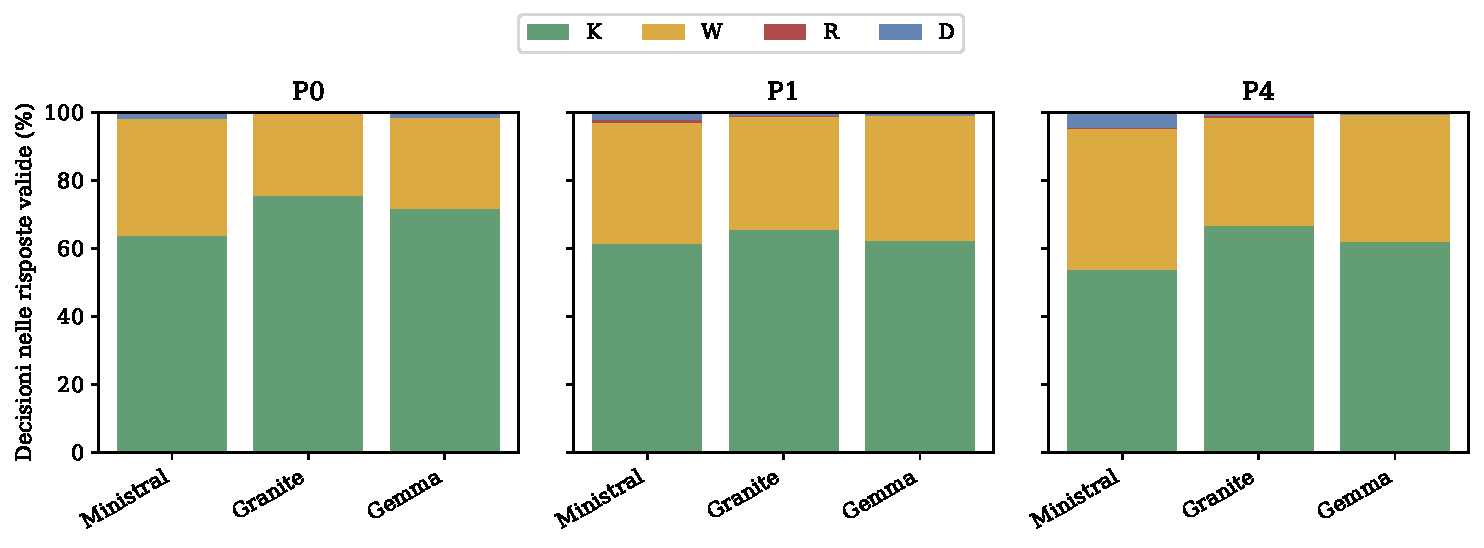
\includegraphics[width=\textwidth]{output/evaluation/evaluator_dynamics_20261026/per_model_actions.pdf}
\caption{Distribuzioni percentuali delle azioni proposte dai modelli. W indica riscrittura e R rimozione. Le differenze non sono misure di accuratezza.}\label{fig:model-action-dynamics}
\end{figure}
Per interpretare i diversi totali occorre considerare anche le risposte
scartate e il numero di rami incontrati nelle run. Il confronto entro
configurazione espone i modelli agli stessi snapshot; fra configurazioni
le gerarchie possono divergere e generare un diverso carico di decisioni.
Una prevalenza di KEEP esprime una tendenza osservata a conservare i padri,
mentre una quota maggiore di REWRITE produce pi\`u proposte di intervento;
nessuna delle due frequenze dimostra, isolatamente, maggiore fedelt\`a documentale.
Nella condizione P4, Ministral propone 366 riscritture e 40 rimozioni
duplicate, contro 281 e 9 di Granite e 314 e 5 di Gemma. In P0 le
riscritture sono rispettivamente 222, 155 e 173. Ministral risulta quindi
pi\`u orientato all'intervento in questi due insiemi di snapshot, mentre
Granite propone pi\`u KEEP. In P1 la distribuzione \`e meno separata:
Gemma propone 222 riscritture, Ministral 218 e Granite 203.
Queste frequenze non vengono estese a input diversi dai casi osservati.
\begin{table}[!htbp]
\centering\small
\caption{Affidabilit\`a del formato globale e retry: richieste finali, risposte valide e tentativi scartati. Un tentativo scartato pu\`o essere seguito da una risposta valida.}\label{tab:model-retry-dynamics}
\begin{tabular}{llrrrr}
\toprule
Config. & Modello & Richieste & Valide & Tentativi & Scartati \\
\midrule
P0 & Ministral & 117 & 117 & 117 & 0 \\
P0 & Granite & 117 & 117 & 117 & 0 \\
P0 & Gemma & 117 & 117 & 124 & 7 \\
P1 & Ministral & 112 & 112 & 112 & 0 \\
P1 & Granite & 112 & 112 & 112 & 0 \\
P1 & Gemma & 112 & 110 & 138 & 28 \\
P4 & Ministral & 113 & 113 & 113 & 0 \\
P4 & Granite & 113 & 113 & 113 & 0 \\
P4 & Gemma & 113 & 109 & 136 & 27 \\
\bottomrule
\end{tabular}
\end{table}
Gli errori registrati sono controlli tecnici o strutturali, non etichette
di scorrettezza semantica. In particolare, una risposta che non copre
esattamente gli ID richiesti viene scartata globalmente: gli altri modelli
non ereditano i suoi voti e non ne compensano i rami mancanti.
Tutti i 62 tentativi scartati di questo insieme riguardano Gemma:
7 in P0, 28 in P1 e 27 in P4. Ministral e Granite non registrano
tentativi scartati nelle run selezionate. Le sei risposte globali
definitivamente invalide non forniscono voti, mentre gli altri errori
sono recuperati entro il budget. Questo dato riguarda affidabilit\`a
del formato nel protocollo adottato, non qualit\`a documentale.

\paragraph{Risposta valida e rispetto delle istruzioni sono distinti.}
La regola KEEP soltanto con EQUIVALENT, riportata nel prompt corrente,
non \`e un vincolo esplicito di \path{_validate_decision}: il codice
controlla la relazione per REMOVE e la disponibilit\`a per REWRITE,
ma non respinge automaticamente KEEP con NOT\_EQUIVALENT.
La Tabella~\ref{tab:keep-relationship-audit} quantifica questi mantenimenti
nelle tracce v111. Si confronta una propriet\`a osservabile delle risposte
con il vincolo documentato; non si ricostruisce da un hash il testo
completo di un prompt storico non salvato. Le azioni rimangono quelle
effettivamente registrate, senza riclassificarle retroattivamente.
\begin{table}[!htbp]
\centering\small
\caption{KEEP con relazione NOT\_EQUIVALENT nelle risposte accettate v111: audit dei dati, distinto dalla correttezza documentale.}\label{tab:keep-relationship-audit}
\begin{tabular}{lrrr}
\toprule
Config. & Ministral & Granite & Gemma \\
\midrule
P0 & 10 & 32 & 6 \\
P1 & 9 & 31 & 3 \\
P4 & 3 & 60 & 3 \\
\bottomrule
\end{tabular}
\end{table}
Il conteggio mostra perch\'e la validit\`a del formato e la maggioranza
non vadano presentate come verifica completa delle condizioni del prompt.
Il codice corrente del validatore \`e riprodotto nel
Listing~\ref{lst:documentary-decision-validator}.
Anche gli altri criteri documentali, come la copertura funzionale del
superstite, richiedono il giudizio semantico e non sono dimostrati dal JSON.

\subsection{Accordo fra modelli e decisioni applicate}
\begin{table}[!htbp]
\centering\small
\caption{Accordo operativo per ramo: unanimit\`a dei tre modelli, quorum senza unanimit\`a, assenza di quorum ed esito finale inconcludente. Il superstite fa parte dell'accordo.}\label{tab:quorum-dynamics}
\begin{tabular}{lrrrrr}
\toprule
Config. & Rami & 3/3 & Quorum 2 & No quorum & Inconcl. \\
\midrule
P0 & 667 & 534 & 107 & 26 & 26 \\
P1 & 617 & 539 & 67 & 11 & 14 \\
P4 & 886 & 660 & 201 & 25 & 27 \\
\bottomrule
\end{tabular}
\end{table}
L'assenza di quorum comprende sia il disaccordo tra voti validi sia
la mancanza di voti utilizzabili. Inoltre il quorum non esaurisce i
controlli: in P1 tre proposte di rimozione duplicata unanimi diventano
inconcludenti perch\'e il superstite non \`e confermato KEEP; lo stesso
accade in due casi P4 con maggioranza di due. Per questo il totale
degli esiti inconcludenti pu\`o superare quello dei soli rami senza quorum.
\begin{table}[!htbp]
\centering\small
\caption{Accordo a coppie sulle operazioni: denominatore limitato ai rami con entrambi i voti validi. Non viene calcolata una misura di correttezza.}\label{tab:pair-agreement-dynamics}
\begin{tabular}{llrr}
\toprule
Config. & Coppia & Confronti & Accordo \\
\midrule
P0 & Granite--Gemma & 646 & 92,4\% \\
P0 & Ministral--Gemma & 646 & 88,9\% \\
P0 & Ministral--Granite & 646 & 83,3\% \\
P1 & Granite--Gemma & 605 & 91,1\% \\
P1 & Ministral--Gemma & 605 & 94,5\% \\
P1 & Ministral--Granite & 614 & 91,4\% \\
P4 & Granite--Gemma & 841 & 87,4\% \\
P4 & Ministral--Gemma & 841 & 87,3\% \\
P4 & Ministral--Granite & 880 & 80,9\% \\
\bottomrule
\end{tabular}
\end{table}
\begin{table}[H]
\centering\small
\caption{Esiti registrati dall'orchestratore per ramo. Gli handoff possono riguardare la stessa generazione batch; non sono conteggi di chiamate o di goal riscritti.}\label{tab:applied-dynamics}
\begin{tabular}{lrrrrr}
\toprule
Config. & KEEP & Handoff & Rimossi & Inconcl. & Preservati \\
\midrule
P0 & 462 & 165 & 6 & 26 & 8 \\
P1 & 381 & 212 & 5 & 14 & 5 \\
P4 & 539 & 312 & 5 & 27 & 3 \\
\bottomrule
\end{tabular}
\end{table}
L'accordo sull'azione non comporta accordo sul contenuto delle critiche.
Un esempio \`e Fitness Tracker, P4, iterazione 1, ramo 4. Tutti i modelli
propongono REWRITE, ma i feedback seguenti orientano diversamente il padre
\emph{Guide beginners through structured and progressive fitness plans}:
\paragraph{Ministral.}
\begin{quote}\small
For 'Guide beginners through structured and progressive fitness plans': the original HLG focuses on beginners, but HLG' emphasizes dynamic adaptation based on user progress. The parent should be restricted to structured onboarding content for beginners while preserving milestone-based progression.
\end{quote}
\paragraph{Granite.}
\begin{quote}\small
For 'Guide beginners through structured and progressive fitness plans': the original HLG implies a one-size-fits-all approach. Rewrite to emphasize adaptability, personalization, and clear milestones for diverse user needs.
\end{quote}
\paragraph{Gemma.}
\begin{quote}\small
For 'Guide beginners through structured and progressive fitness plans': the reconstruction (HLG') suggests dynamic adaptation based on progress, but the original HLG focuses on onboarding and step-by-step routines. The project description emphasizes providing structured plans and guidance for beginners to build confidence. The rewrite should preserve the onboarding and step--by-step routines while incorporating the dynamic adaptation mentioned in the reconstruction.
\end{quote}
La maggioranza approva dunque l'intervento, senza risolvere automaticamente
la tensione fra restringere l'onboarding ai principianti ed estendere
adattabilit\`a e personalizzazione. Il generatore riceve le critiche concordi
sull'azione, anche quando la loro formulazione non \`e pienamente compatibile.
Questo caso spiega un limite concreto del quorum e del feedback concatenato;
non dimostra da solo la causa di tutte le variazioni di F1 del dataset.

\subsection{Convergenza, stabilit\`a dello stato e costo iterativo}
\begin{table}[!htbp]
\centering\small
\caption{Arresto e modifiche nella suite v111. Le visite ripetute contano soltanto un ritorno esatto a uno stato gi\`a visto dopo una modifica; le iterazioni senza modifica sono separate.}\label{tab:state-dynamics}
\begin{tabular}{lrrrrrr}
\toprule
Config. & Conv. & Iterazioni & Media & Modifica & Invariate & Ritorni \\
\midrule
P0 & 10/12 & 117 & 9,75 & 64 & 53 & 0 \\
P1 & 11/12 & 112 & 9,33 & 74 & 38 & 0 \\
P4 & 10/12 & 113 & 9,42 & 87 & 26 & 0 \\
\bottomrule
\end{tabular}
\end{table}
\begin{table}[!htbp]
\centering\small
\caption{Iterazioni per dataset e configurazione. Il simbolo $\dagger$ indica arresto al limite di 25 senza convergenza; gli altri valori indicano conferma di tutti i rami.}\label{tab:dataset-iteration-dynamics}
\begin{tabular}{lrrr}
\toprule
Dataset & P0 & P1 & P4 \\
\midrule
AUU & 25$^{\dagger}$ & 21 & 25$^{\dagger}$ \\
Calculator & 1 & 1 & 1 \\
Ethical Purchasing & 1 & 1 & 1 \\
Event Organization & 3 & 9 & 2 \\
Fitness Tracker & 6 & 15 & 16 \\
Genome Nexus & 1 & 1 & 1 \\
Gestao Hospital & 1 & 1 & 1 \\
La Reine Marlene & 7 & 3 & 8 \\
London Ambulance & 13 & 16 & 5 \\
Planning Poker & 25$^{\dagger}$ & 8 & 4 \\
Recycling & 10 & 11 & 24 \\
SIA 25--26 & 24 & 25$^{\dagger}$ & 25$^{\dagger}$ \\
\bottomrule
\end{tabular}
\end{table}
\begin{figure}[htbp]
\centering
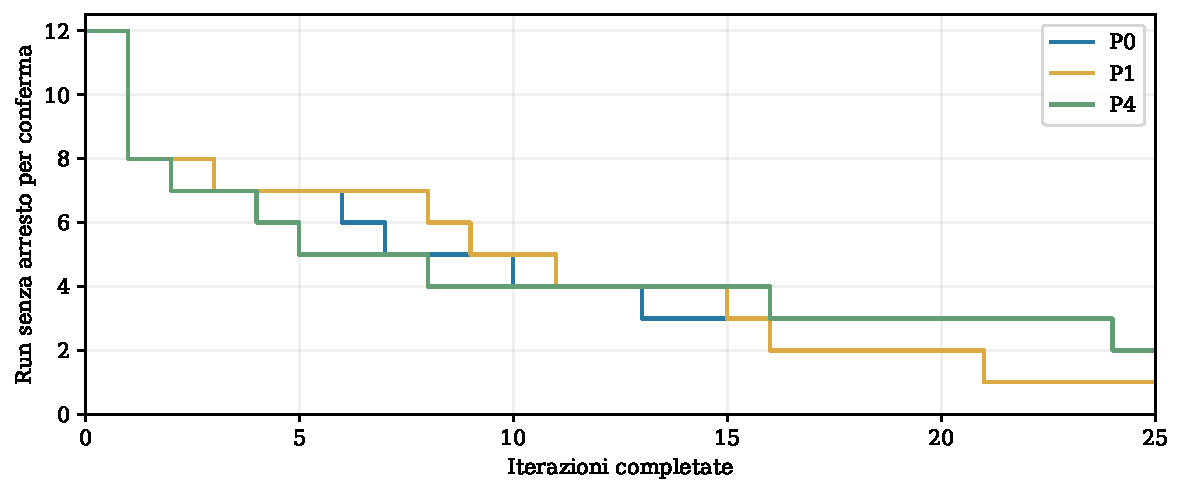
\includegraphics[width=\textwidth]{output/evaluation/evaluator_dynamics_20261026/confirmation_curves.pdf}
\caption{Run non ancora arrestate per conferma dopo ciascuna iterazione. A 25 restano rappresentate le run terminate al limite: il loro completamento tecnico non equivale a convergenza.}\label{fig:confirmation-dynamics}
\end{figure}
Le iterazioni prive di cambiamenti non implicano necessariamente arresto:
possono rimanere riscritture che riproducono lo stesso testo, voti senza
quorum o aggiornamenti rifiutati. Viceversa, un handoff completato non
garantisce una modifica effettiva del contenuto. I ritorni esatti a stati
precedenti costituiscono un indicatore restrittivo di ciclicit\`a; una
serie di parafrasi differenti non viene classificata come lo stesso stato.
I soli conteggi aggregati delle azioni non dimostrano pertanto l'oscillazione
di un particolare goal.
In queste tracce non compaiono ritorni esatti a uno stato precedente
dopo una modifica. Si osservano per\`o 53 iterazioni senza variazioni
in P0, 38 in P1 e 26 in P4. La mancata convergenza non va quindi
descritta automaticamente come ciclo tra due gerarchie identiche:
pu\`o comprendere stasi o una successione di formulazioni differenti.
Nel riferimento P4 AUU e SIA 25--26 raggiungono il limite, mentre
Recycling converge solo alla ventiquattresima iterazione e Fitness
Tracker alla sedicesima.

La convergenza resta un criterio operativo e non una certificazione della
gerarchia. I risultati finali di F1 sono misurati anche per le run non
convergenti: eliminarle favorirebbe artificialmente i casi pi\`u semplici.
Le run lunghe producono molte osservazioni correlate dello stesso progetto,
che non diventano repliche indipendenti. Per questo le tabelle dei voti
usano conteggi di processo, mentre le metriche finali continuano ad
attribuire lo stesso peso ai dodici dataset.
